\documentclass[11pt]{amsart}
\usepackage{amsmath,amssymb,mathtools}
\usepackage[T1]{fontenc}
\usepackage{lmodern,microtype,booktabs,tikz}
\usepackage{xurl}
\usepackage[hidelinks]{hyperref}
\usepackage[nameinlink,noabbrev]{cleveref}
\newtheorem{theorem}{Theorem}[section]
\newtheorem{lemma}[theorem]{Lemma}
\newtheorem{proposition}[theorem]{Proposition}
\newtheorem{corollary}[theorem]{Corollary}
\theoremstyle{definition}
\newtheorem{definition}[theorem]{Definition}
\theoremstyle{remark}
\newtheorem{remark}[theorem]{Remark}
\newtheorem{example}[theorem]{Example}
\newtheorem{mainq}{Theorem}
\renewcommand{\themainq}{Q}
\newtheorem{mainr}{Theorem}
\renewcommand{\themainr}{R}
% Declare names explicitly, including types that share the theorem counter.
\crefname{theorem}{Theorem}{Theorems}
\Crefname{theorem}{Theorem}{Theorems}
\crefname{lemma}{Lemma}{Lemmas}
\Crefname{lemma}{Lemma}{Lemmas}
\crefname{proposition}{Proposition}{Propositions}
\Crefname{proposition}{Proposition}{Propositions}
\crefname{corollary}{Corollary}{Corollaries}
\Crefname{corollary}{Corollary}{Corollaries}
\crefname{definition}{Definition}{Definitions}
\Crefname{definition}{Definition}{Definitions}
\crefname{example}{Example}{Examples}
\Crefname{example}{Example}{Examples}
\crefname{section}{Section}{Sections}
\Crefname{section}{Section}{Sections}
\crefname{appendix}{Appendix}{Appendices}
\Crefname{appendix}{Appendix}{Appendices}
\crefname{mainq}{Theorem}{Theorems}
\Crefname{mainq}{Theorem}{Theorems}
\crefname{mainr}{Theorem}{Theorems}
\Crefname{mainr}{Theorem}{Theorems}

% Keep Lean identifiers intact and let the surrounding prose wrap.
\newcommand{\leanid}[1]{\mbox{\ttfamily\detokenize{#1}}}
\newcommand{\R}{\mathbb R}
\newcommand{\Q}{\mathbb Q}
\newcommand{\dt}{\,\mathrm{d}t}
\newcommand{\FaceLP}{\textsc{FaceLP}}
\DeclareMathOperator{\argmin}{arg\,min}
\DeclareMathOperator{\conv}{conv}
\DeclareMathOperator{\cost}{cost}

\title[Exact optimization of weighted mean busy dates]{Exact Polynomial-Time Optimization of Weighted Mean Busy Dates on Identical Parallel Machines}
\author{The Blank Beyond}
\date{27 November 2026 (revised)}
\subjclass[2020]{90B35, 90C05, 90C25}
\keywords{mean busy date, preemptive scheduling, parallel machines, exact bit complexity, continuous linear programming, formal verification}
\hypersetup{pdfauthor={The Blank Beyond},pdftitle={Exact Polynomial-Time Optimization of Weighted Mean Busy Dates on Identical Parallel Machines},pdfsubject={Research manuscript (preliminary finding)},pdfkeywords={mean busy dates, preemption, exact optimization, identical parallel machines}}
\raggedbottom
\begin{document}
\begin{abstract}
We consider preemptive scheduling on identical parallel machines with migration, positive rational workloads and objective coefficients, and all jobs available at time zero. The objective is a weighted sum of job processing-time first moments. We give a deterministic algorithm with weakly polynomial Turing bit complexity when the machine count is part of the input. It returns an exact optimum over feasible measurable schedules on the half-line. An exact linear program tests membership in the dual minimizer set, and a rational description bound permits recovery by strong separation. A reflected row-wrapping construction realizes the optimal constant allocations while preserving each job's workload and first moment. The realization theorem and the soundness of an executable rational optimality checker are verified in Lean. The optimization and its bit-complexity analysis are proved conventionally.
\end{abstract}
\maketitle
\section{Introduction}\label[section]{sec:intro}

When cost accrues throughout processing, it depends on when each fraction of a job is served. We study a positively weighted sum of first processing moments, where a job's moment is the integral of time over the set on which it runs. The machines are identical and allow preemption and migration, and all jobs are available at time zero. A job may occupy at most one machine at a time.

Queyranne posed the complexity question for this model in 2010 \cite[pp.~15--17]{queyranne2010}. The note describes a fixed-machine convex quadratic formulation with a variable for each feasible job subset. The number of subsets of size at most $m$ is polynomial in $n$ for fixed $m$, but can be exponential in $n$ when $m$ varies. An algorithm with a polynomial binary-time bound for a variable machine count must avoid that enumeration.

We prove such a bound and give an algorithm returning rational schedule records and a rational certificate of the exact optimum. We first relax binary activities to bounded fractional rates. Sorting score zeros and crossings allows exact integration of the support function of the rate polytope. A linear feasibility problem tests dual optimality even at tied scores. A description bound for the polytope of dual minimizers then enables exact strong optimization in the framework of Gr\"otschel, Lov\'asz and Schrijver \cite{gls1988}. The description bound uses a rational quadratic representation on each parameter cell. The algorithm needs neither the full arrangement nor a time discretization. A second result gives an explicit finite schedule from the optimal rates. Its reflection step preserves the first moment of each job, as well as its work.

\Cref{sec:model} specifies the model and results. Attained duality, the minimizer polytope, exact recovery and unrestricted optimality are developed in \Cref{sec:dual,sec:separation,sec:recovery}. The realization and the exact certificate for Queyranne's example are in \Cref{sec:realization,sec:example}. The explicit bit bounds and imported optimization contracts appear in \Cref{app:encoding,app:gls}. \Cref{sec:formal} explains the scope of the Lean proofs.

\section{Related work}\label[section]{sec:related}

\paragraph{Scheduling.}
Goemans \cite{goemans1997} used mean busy times in approximation algorithms for scheduling with release dates. Subsequent work analyzed linear relaxations through this objective \cite{goemans2002}. Related uses include approximation algorithms for weighted completion time on unrelated machines \cite{sitters2017} and completion-time scheduling with job assignments to machines \cite{sethuraman1999}. A job's completion time is the end of its processing. The objective here depends on all processing times, through an integral. Queyranne's fixed-machine result is attributed to his unpublished notes of 20 July 2010, identified in the proceedings note \cite[discussion~3 and ref.~4]{queyranne2010}. Those notes were unavailable for direct comparison.

J\"ager, Lindermayr and Megow \cite{jaeger2026} use a time-indexed weighted mean-busy-time relaxation to bound weighted completion time in polytope scheduling. Damerius, Kling and Schneider \cite{damerius2024} use fractional total completion time in a continuous LP to obtain a completion-time lower bound and an approximation guarantee for scheduling with a shared resource. Here the continuous first moment is itself the objective, and the algorithm recovers an exact optimum and an attaining schedule for identical machines.

\paragraph{Separated continuous linear programming.}
The fractional problem for a fixed horizon is an instance of the linear-data separated continuous linear program (SCLP) studied by Weiss \cite{weiss2008}. To see this, write $U_j(t)=\int_0^t u_j(s)\,\mathrm{d}s$ and impose the pointwise rate and total capacity constraints, introducing nonnegative slacks if needed. The cumulative rows can be written
\[
 U_j(t)\leq p_j,\qquad -U_j(t)\leq H-p_j-t .
\]
They follow from the terminal workloads and $0\leq u_j\leq1$, and they force $U_j(H)=p_j$. Maximizing $\int_0^H(H-t)\alpha\cdot u(t)\dt$ for these controls differs from minimizing the processing cost by the fixed term $H\alpha\cdot p$. Thus the continuous model already fits established machinery.

Weiss gives a simplex-based finite-step method. The author-posted revision bounds the number of pivots combinatorially under its feasibility and nondegeneracy hypotheses. A worst-case polynomial Turing bit bound would require polynomial control of both the number of steps and their bit costs in the variable-machine input size. Finite termination alone leaves both estimates open, and the literature examined did not supply that bound for this scheduling specialization. Shindin and Weiss extend simplex-type finite termination to a measure-valued continuous linear program with constant coefficients that includes SCLP \cite{shindinweiss2020}. Their general analysis allows exponential worst-case behavior. An implementation of a revised SCLP simplex is studied in \cite{shindin2021}. Its numerical results concern practical performance. Fleischer and Sethuraman give a polynomial approximation scheme with additive and multiplicative tolerances for a more general holding-cost formulation \cite{fleischer2005}. For any feasible half-line control, Tonelli's theorem gives $\int_0^\infty t u_j(t)\dt=\int_0^\infty(p_j-U_j(t))\dt$, which explains the holding-cost interpretation. The result here concerns exact rational recovery with polynomial worst-case bit time.

\paragraph{Purification and explicit realization.}
For a constant rate vector, decompose it into a distribution on the finite set of binary feasible job patterns. Classical finite-action atomless purification preserves the probability assigned to each pattern under both time measure and first-moment measure \cite[\S2]{dww1950}. On a signed interval use $(t-a)\dt$ for the second measure and recover the signed moment using the preserved work. Summing over the patterns containing a job preserves that job's work and first moment. This already gives measurable existence. The publisher's abstract of Anderson and Pullan \cite{andersonpullan1996} describes a constructive SCLP purification to an extreme point without decreasing the objective. The full text was unavailable for comparing its construction, precise hypotheses, and rational operation bounds. The realization proved here uses McNaughton's row wrap \cite[Theorem~3.1]{mcnaughton1959} on a half-interval and then reflects the operations. It gives explicit machine assignments and a finite rational output with a per-job record bound.

\paragraph{Optimization tools and scope of comparison.}
Parameter-dependent affine orderings and polyhedral descriptions are standard themes in parametric optimization \cite{nemesch2025}. Given the fixed-machine pattern formulation, a natural route is to dualize the $n$ workload constraints and seek exact recovery through the framework of Gr\"otschel, Lov\'asz and Schrijver \cite{gls1988}. With standard convex duality \cite{rockafellar1970}, the problem-specific steps are to describe the minimizers of an \emph{integrated} support function by polynomial-size rational rows, supply an exact workload-based separator, and turn the resulting rates into a moment-preserving schedule. The literature examined established prior continuous formulations, finite-step algorithms, and measurable purification. It did not identify the full variable-machine worst-case polynomial bit guarantee in \Cref{thm:q}. The unpublished notes, the uninspected portions of the purification literature, and the scope of the bibliographic coverage leave priority unresolved.

\section{Model and main theorems}\label[section]{sec:model}

There are $n\geq 1$ jobs with workloads $p_j\in\Q_{>0}$, coefficients $\alpha_j\in\Q_{>0}$, and $m\geq1$ identical unit-speed machines. Jobs are available at time zero. A schedule consists of measurable job assignments to the machines on $[0,\infty)$, with an idle assignment allowed. At almost every time each job is assigned to at most one machine. Write $\sigma_j(t)\in\{0,1\}$ for its activity indicator. The workloads and objective are
\begin{equation}\label{eq:model}
 \int_0^\infty \sigma_j(t)\dt=p_j\quad(1\leq j\leq n),\qquad
 \cost(\sigma)=\sum_{j=1}^n\alpha_j\int_0^\infty t\sigma_j(t)\dt .
\end{equation}
Preemption and migration are unrestricted. The cost may take the value $+\infty$. Equivalently, one can specify measurable binary activities with $\sum_j\sigma_j\leq m$ almost everywhere. Indeed, assign the active job indices in increasing order to the first available machines at each time, making all machines idle on an exceptional null set. This assignment is measurable because there are finitely many active subsets. Both representations permit arbitrary measurable changes of activity.

Queyranne's displayed $M_j$ is the raw integral $\int_0^\infty t\sigma_j(t)\dt$ \cite[p.~15]{queyranne2010}. For the normalized convention $\bar M_j=M_j/p_j$, the weighted objective $\sum_j w_j\bar M_j$ has coefficients $\alpha_j=w_j/p_j$. Conversely, the normalized weights corresponding to raw coefficients $\alpha_j$ are $w_j=\alpha_jp_j$.

The algorithm uses an explicit list of jobs, a positive binary integer $m$, and binary numerator--denominator pairs for the rational data. Let $L$ be the entire bit length, including framing. A finite output schedule consists of job and machine indices and rational half-open operation intervals $[s,e)$ with $0\leq s<e$. The schedule idles elsewhere. In the optimization proof put $m_\star=\min(m,n)$.

\begin{mainq}[Exact optimization]\label[mainq]{thm:q}
For every instance of \eqref{eq:model}, a deterministic algorithm returns an exact rational optimum, a globally optimal finite schedule with rational endpoints, and a rational dual certificate verifiable in polynomial bit time. The algorithm is weakly polynomial, using a number of Turing bit operations polynomial in $L$ with $m$ part of the input. Global optimality is over the feasible measurable schedules on $[0,\infty)$. There are $O(n^3)$ nonempty operation records and global event intervals up to the certificate horizon, or $O(n^4)$ entries when every active job and machine is listed on each such interval. The endpoint lengths and the entire output encoding are polynomial in $L$.
\end{mainq}

\begin{mainr}[Reflected realization]\label[mainr]{thm:r}
Let $m,n\geq1$. For each of $q$ consecutive rational intervals $[a_\ell,b_\ell]$, $a_\ell\leq b_\ell$, let $z_\ell\in\Q^n$ satisfy
\[
 0\leq z_{\ell j}\leq1,\qquad \sum_{j=1}^n z_{\ell j}\leq m .
\]
There is an explicit finite rational realization on at most $\min(m,n)$ machines, with no machine or job overlap, such that for each interval and job
\begin{equation}\label{eq:target-moments}
 \int_{a_\ell}^{b_\ell}\sigma_j(t)\dt=(b_\ell-a_\ell)z_{\ell j},\qquad
 \int_{a_\ell}^{b_\ell}t\sigma_j(t)\dt
      =\tfrac12(b_\ell^2-a_\ell^2)z_{\ell j}.
\end{equation}
The construction uses at most $4nq$ nonempty operation records and is computable in polynomial bit time in the explicit allocation encoding. It applies on the real line for rational shifts and gives a schedule in the model above when the intervals are nonnegative. The bound on global event intervals is $O(nq)$ and the expanded assignment representation has size $O(n^2q)$ entries.
\end{mainr}

The proof of \Cref{thm:q}, including exact rational recovery and the binary complexity analysis, is conventional. The construction, feasibility, workload and moment identities, and record bound of \Cref{thm:r} are machine-checked. The associated checker theorem and the relation between the executable and measurable models are described in \Cref{sec:formal}.

\section{Continuous relaxation and attained duality}\label[section]{sec:dual}

Set $V=\sum_jp_j$, $H=2V$, and
\[
 P=\{u\in[0,1]^n:\ \textstyle\sum_j u_j\leq m_\star\}.
\]
The relaxation allows measurable rates $u(t)\in P$ with the original workloads. Its cost is $C(u)=\int t\,\alpha\cdot u(t)\dt$ over the specified horizon. All feasible schedules induce such controls.

\begin{lemma}[Time compression and multiplier bounds]\label[lemma]{lem:compression}
The relaxed minimum over the half-line is attained by a control vanishing after $V$. For
\begin{equation}\label{eq:f}
 h_P(c)=\max_{v\in P}c\cdot v,\qquad
 J(\lambda)=\int_0^H h_P(\lambda-t\alpha)\dt,\qquad
 f(\lambda)=J(\lambda)-\lambda\cdot p,
\end{equation}
the set $K^*=\argmin_{\lambda\in\R^n} f(\lambda)$ is nonempty, contained in $K=\prod_j[0,\alpha_jV]$, and the relaxed minimum is $-\min f$. At any pair of primal and dual optima the control maximizes the support integrand almost everywhere on $[0,H]$.
\end{lemma}

\begin{proof}
We first compress feasible controls without increasing cost, then use finite-horizon attainment and the workload value function to obtain and bound the multipliers.

For a feasible half-line control put $r(t)=\sum_j u_j(t)$, $\rho(t)=\min(1,r(t))$ and $s(t)=\int_0^t\rho(a)\,\mathrm{d}a$. The clock $s$ is absolutely continuous, satisfies $s(t)\leq t$, and tends to $S=\int_0^\infty\rho(t)\dt\leq V$. It pushes the measure $\rho(t)\dt$ onto Lebesgue measure on $(0,S)$. For $0<x<S$ the mass of the preimage of the initial segment $(0,x)$ is $x$, by continuity of the clock and its definition as a cumulative integral. Initial segments determine the pushforward. The generalized inverse $\tau(v)=\inf\{t\geq0:s(t)\geq v\}$ satisfies $\tau(s(t))=t$ for $\rho(t)\dt$-almost every $t$. The nontrivial levels of $s$ are intervals with zero $\rho(t)\dt$ mass and there are at most countably many, since their interiors are disjoint. The endpoint levels $0,S$ also have zero mass. We can take Borel representatives of the measurable rates and modify them on null sets.

On the new clock use $u_j(\tau(v))/\rho(\tau(v))$ where the denominator is positive and zero on the exceptional set and after $S$. The pushforward and inverse identities show that the denominator is positive almost everywhere on $(0,S)$. If $0<r\leq1$, the new rates are nonnegative and sum to one. If $r>1$ they are unchanged. Thus they are in $P$. Their workloads are the original ones. The new first moments are $\int_0^\infty s(t)u_j(t)\dt\leq\int_0^\infty t u_j(t)\dt$, using nonnegative integration even for infinite original moments. Consequently the half-line infimum equals the infimum on $[0,H]$, using in the other direction extension by zero.

On $[0,H]$ the $P$-valued controls form a weak-$*$ closed subset of a bounded ball in $L^\infty([0,H];\R^n)$. Indeed, each linear rate constraint holds almost everywhere exactly when it holds in integrals against every nonnegative $L^1$ test function. Workloads and cost are weak-$*$ continuous, so Banach--Alaoglu gives attainment on any nonempty workload fiber. The set of workloads is $HP$, by convexity in one direction and the constant control in the other. Write $W(v)$ for the minimum at workload $v\in HP$. It is finite and convex, by convex combinations of minimizing controls. Since $0<p_j<H$ and $V<MH$, the workload $p$ is in the interior of $HP$. By the supporting subgradient theorem for a finite convex function at such a point \cite[Theorem~23.4]{rockafellar1970}, there is $\lambda$ with
\[
 W(v)\geq W(p)+\lambda\cdot(v-p)\qquad(v\in HP).
\]
For every control without a workload constraint, $C(u)-\lambda\cdot\int u\geq W(p)-\lambda\cdot p$, and an optimum at $p$ achieves equality. The unconstrained infimum is $-J(\lambda)$. A pointwise maximizer of the support is measurable by choosing among finitely many vertices with a fixed tie order, or by the envelope in \Cref{lem:envelope}. Weak duality for every multiplier follows by integrating the same support inequality at workload $p$. This proves dual attainment and the claimed equality. At any pair of optima the nonnegative support deficit integrates to zero, which gives complementarity. Conversely, a control of workload $p$ with zero deficit almost everywhere attains the dual bound.

Compress a primal optimum and extend it by zero after $V$. It remains optimal since the minimum over the half-line equals $W(p)$. Complementarity with any $\lambda\in K^*$ gives $h_P(\lambda-t\alpha)=0$ almost everywhere on $(V,H)$. Each coordinate unit vector belongs to $P$, so $\lambda_j\leq\alpha_j V$. If $\lambda_j\leq0$, job $j$ has strictly negative score at every $t>0$. Deleting its positive rate strictly improves any pointwise maximizer with positive $j$-th coordinate, contradicting the positive required workload. Hence $K^*\subseteq K$.
\end{proof}

\section{Strong separation and the minimizer polytope}\label[section]{sec:separation}

\begin{lemma}[Support envelope]\label[lemma]{lem:envelope}
For $c\in\R^n$, $h_P(c)$ sums the at most $m_\star$ largest positive entries of $c$. For fixed $\lambda$, there are at most $q_0=1+n(n+1)/2$ intervals on which a fixed binary vector supports $\lambda-t\alpha$. Their endpoints and a maximizing binary vector on each interval can be found by rational arithmetic for rational $\lambda$.
\end{lemma}

\begin{proof}
If two coordinates of a point in $P$ are fractional, transferring a sufficiently small amount between them in both directions disproves extremality. A lone fractional coordinate can be perturbed in both directions when capacity is slack. When capacity is tight, integrality of capacity and of the remaining coordinates makes the last coordinate integral. The feasible binary vectors are vertices already in the cube. Selecting the largest positive scores, up to capacity, maximizes over these vertices.

Include $0,H$, every zero $Z_i=\lambda_i/\alpha_i$, and every crossing $C_{ij}=(\lambda_i-\lambda_j)/(\alpha_i-\alpha_j)$ for $i<j$ and $\alpha_i\ne\alpha_j$. Keep interior events together with the endpoints, sort, and remove duplicates. Let $I_\ell=(a_\ell,b_\ell)$, $1\leq\ell\leq r$, denote the resulting intervals and $\Delta_\ell=b_\ell-a_\ell$. The signs and order of affine scores are constant on each $I_\ell$. Equal slopes give a constant order or identical scores. At its midpoint $s_\ell$ choose a support vertex $v_\ell$ using job indices to break ties. It maximizes the support throughout $I_\ell$ and at its endpoints by continuity. The bound on $r$ counts zeros and crossings. This procedure sorts $O(n^2)$ time events and at most $n$ scores in each interval.
\end{proof}

One obtains the integral by summing
\begin{equation}\label{eq:integral-piece}
 (\lambda\cdot v_\ell)\Delta_\ell
 -\tfrac12(\alpha\cdot v_\ell)(b_\ell^2-a_\ell^2).
\end{equation}

\begin{lemma}[Exact membership and separation]\label[lemma]{lem:separate}
There is a rational strong separation oracle for $K^*$ with runtime polynomial in $L$ and the binary length of its query.
\end{lemma}
\begin{proof}
For a fixed query $\lambda$ use \Cref{lem:envelope} and let
\[
 F_\ell=\{z\in P:(\lambda-s_\ell\alpha)\cdot z
                    =(\lambda-s_\ell\alpha)\cdot v_\ell\}.
\]
On $I_\ell$ the maximizing face is exactly $F_\ell$. For each vertex of $P$ its deficit relative to $v_\ell$ is affine and nonnegative on $I_\ell$. A zero at an interior point forces this affine function to vanish throughout. Taking convex hulls gives the assertion for the entire face, including persistent ties.

Solve the rational feasibility linear program
\begin{equation}\label{eq:facelp}
 \FaceLP(\lambda):\qquad
 z_\ell\in F_\ell\quad(1\leq\ell\leq r),\qquad
 \sum_{\ell=1}^r \Delta_\ell z_\ell=p .
\end{equation}
If feasible, the constant rates on these intervals meet the workloads and are complementary. Thus $\lambda\in K^*$. Conversely, if $\lambda\in K^*$, a complementary optimum exists by \Cref{lem:compression}, and averaging it over each interval gives feasible $z_\ell$ because $F_\ell$ is convex.

If the query lies outside $K$, a coordinate normal for a violated bound strictly separates it from $K^*$. Inside $K$, first solve \eqref{eq:facelp} and accept membership on feasibility. Otherwise put $g=\sum_\ell\Delta_\ell v_\ell-p$. Using $v_\ell$ in \eqref{eq:f} at a different multiplier gives $f(x)\geq f(\lambda)+g\cdot(x-\lambda)$. Therefore
\[
 g\cdot(\lambda-x)\geq f(\lambda)-f(x)>0\qquad(x\in K^*).
\]
Nonemptiness implies $g\ne0$. Return the rational normal $g/\|g\|_\infty$. The membership test is essential because an arbitrarily selected support vertex can yield a nonzero subgradient even at a minimizer. \Cref{app:encoding} establishes the oracle's exact bit bounds, including the explicit LP call.
\end{proof}

\begin{lemma}[Rational minimizer polytope]\label[lemma]{lem:polytope}
The set $K^*$ is a rational polytope of polynomial facet complexity in the GLS whole-row convention. The bound can be computed from $L$ and $n$ without generating its faces or vertices.
\end{lemma}

\begin{proof}
\emph{Arrangement and closure.}
Use the following equality loci in the full multiplier space.
\begin{enumerate}
 \item $Z_i=Z_j$ for two zero events.
 \item $Z_i=C_{jk}$ and $C_{ij}=C_{kl}$ for mixed and pair-crossing comparisons, with crossings defined only for nonparallel scores.
 \item $A=0$ and $A=H$ for every zero or crossing event $A$.
 \item $\lambda_i=\lambda_j$ when $\alpha_i=\alpha_j$.
 \item $\lambda_j=0$ and $\lambda_j=\alpha_jV$ for the box.
\end{enumerate}
An identical equality represents a persistent comparison, and a constant impossible equality gives a fixed strict order. Discard both from the wall list. There are $O(n^4)$ proper hyperplanes, with polynomial rational row encodings as shown in \Cref{app:encoding}. Their complement is dense. The nonempty strict sign chambers are open and full dimensional. Every point is in a chamber closure, by taking a sequence in the complement and a subsequence of one sign pattern. The closure of a nonempty chamber is the corresponding weak system. A convex combination of any point of the weak system and a fixed chamber point, with positive weight on the latter tending to zero, gives the required approximation. The intersections $C$ of closed chambers with $K$ cover the box.

\emph{Quadratic pieces.}
Inside an open chamber the retained events, their order, and the support vector on each event interval are fixed as a combinatorial selection. The sign of a score is the sign of $Z_i-t$, the nonparallel difference has the sign of $(\alpha_i-\alpha_j)(C_{ij}-t)$, and the parallel order is fixed by the fourth type of comparison. Thus the endpoints in \eqref{eq:integral-piece} are fixed rational affine functions of $\lambda$ and the $v_\ell$ are fixed binary vectors. Integrating and subtracting $\lambda\cdot p$ yields a rational quadratic
\[
 q_C(x)=\tfrac12 x^TQ_Cx+d_C\cdot x+e_C
\]
with symmetric $Q_C$. Convexity of $f$ follows from \eqref{eq:f}. Second differences on sufficiently short segments through an interior point of the open chamber imply $v^TQ_Cv\geq0$ for every direction $v$. Since both functions are continuous, the polynomial agrees with $f$ on the whole closure and hence on $C$, including coincident events and lower-dimensional intersections.

\emph{Rational cell minima.}
Write a nonempty clipped chamber as $C=\{x:Ax\leq b\}$. It is compact. At a minimum the negative gradient lies in the cone of active outward row normals. In fact any direction satisfying the active directional inequalities is feasible for small positive steps. The gradient is nonnegative on such directions. The polar of these directions is the cone of active normals, by finite-dimensional separation for finitely generated cones \cite[Sections~19 and~22]{rockafellar1970}. Conic Carath\'eodory gives at most $n$ normals, indexed by $I$. To obtain this bound one can start with any conic representation and, if its positive support is dependent, subtract a multiple of one dependence until a coefficient vanishes, with all coefficients remaining nonnegative. The resulting nonempty rational system is
\begin{equation}\label{eq:kkt}
 Ax\leq b,\quad A_Ix=b_I,\quad
 Q_Cx+d_C+A_I^T\mu=0,\quad \mu\geq0 .
\end{equation}
Every solution gives a cell minimizer, by the first-order inequality for the convex quadratic and the multiplier signs. This system is pointed. A line would have zero $x$-direction by boundedness and zero $\mu$-direction by nonnegativity along the entire line. Its dimension is at most $2n$ in the ambient variables, and the rational vertex bound in \Cref{app:encoding} furnishes a rational minimizer $x_C$ of polynomial encoding length.

For $x\in C$,
\[
 q_C(x)-q_C(x_C)
 = (Q_Cx_C+d_C)\cdot(x-x_C)+\tfrac12(x-x_C)^TQ_C(x-x_C).
\]
Both terms are nonnegative. The quadratic term vanishes precisely on the Hessian kernel. Thus the whole cell minimizer polytope $S_C$ is specified by $Ax\leq b$ and
\begin{equation}\label{eq:cell-min}
 Q_C(x-x_C)=0,\qquad (Q_Cx_C+d_C)\cdot(x-x_C)=0 .
\end{equation}
These equations allow minima through the interior of a cell. Their row lengths and those of the resulting vertices admit uniform polynomial bounds.

\emph{Global minimum.}
For $f_*=\min f$, coverage and equality on each cell give
\[
 K^*=\bigcup_{\substack{C\ne\varnothing\\ \min_C q_C=f_*}} S_C .
\]
The compact set $K^*$ is convex by convexity of $f$. The finite union of the qualifying polytopes is therefore the convex hull of their combined vertex lists. Each vertex of $K^*$ belongs to one of those lists, since an extreme point cannot be a proper convex combination of distinct points of $K^*$. The uniform vertex-length bound and GLS Lemma~(6.2.4)(b) give the whole-row description bound in \Cref{app:encoding}, with no condition on the affine dimension. The cells and their KKT systems enter only the description proof. The algorithm uses the oracle of \Cref{lem:separate}.
\end{proof}

\section{Exact recovery and optimality on the half-line}\label[section]{sec:recovery}

Apply strong linear optimization to the well-described polytope $K^*$, with exact strong separation from \Cref{lem:separate} and a computable row-length promise from \Cref{lem:polytope}. The requisite GLS results, including their lower-dimensional contracts, are stated in \Cref{app:gls}. Use at most $n$ calls to minimize successive coordinates of a multiplier, imposing each attained value as an equality before the next call. Each restriction is a nonempty exposed face of its predecessor, and its vertices are original vertices of $K^*$. To separate a query violating a fixed coordinate use a signed coordinate vector. For the other queries the original separation oracle suffices. The final surviving point $\lambda^*$ is rational, lies in $K^*$, and has the vertex encoding bound. The zero-coordinate padding in \Cref{app:encoding} gives the uniform oracle convention. Alternatively the GLS feasibility result alone would give a rational multiplier.

Build \eqref{eq:facelp} at $\lambda^*$. This is a nonempty bounded explicit LP. Minimize and fix successive rate coordinates by exact rational LP, giving a vertex $z^*$ after at most $nr$ calls. This supplies rates complementary to the dual and with workload $p$. Apply \Cref{thm:r} on the corresponding $r$ intervals and idle after $H$. The workload and individual first moments are preserved, so the schedule attains the relaxed minimum.

For any feasible half-line schedule, the bound $\lambda^*_j\leq\alpha_jV$ implies $\lambda^*_j-t\alpha_j\leq0$ for $t\geq H$. The support is zero on the tail because $P$ contains zero and has nonnegative coordinates. The pointwise inequality
\[
 (\lambda^*-t\alpha)\cdot\sigma(t)\leq h_P(\lambda^*-t\alpha)
\]
then gives
\begin{equation}\label{eq:bound}
 \cost(\sigma)\ \geq\ \lambda^*\cdot p-J(\lambda^*) .
\end{equation}
For finite cost both sides of the integrated pointwise comparison are justified by finite workloads and the compactly supported envelope. For infinite cost the finite lower bound holds immediately. Thus no restriction on the competitors' finishing times is needed. The constructed schedule attains equality in \eqref{eq:bound}. More generally the same certificate argument works with any supplied rational horizon $H$ satisfying $\lambda_j-H\alpha_j\leq0$ for all $j$ and with exact primal--dual equality.

\paragraph{Algorithm.}
\begin{enumerate}
\item Form the raw coefficients, horizon, box and row-length bound in \Cref{app:encoding}.
\item Recover $\lambda^*$ by successive strong optimization. For each query check the imposed coordinate constraints and box, build the support envelope, solve \eqref{eq:facelp}, and return membership or the separating normal from \Cref{lem:separate}.
\item Build the final \FaceLP{} and obtain a rate vertex by successive exact LP minimization.
\item Use reflected wrapping on the constant-rate intervals. Return the schedule, exact cost and multiplier.
\end{enumerate}

An exact certificate verifier checks machine and job nonoverlap, workloads, rational moments and cost by an event sweep. It checks the tail condition and integrates $h_P$ using the envelope, or checks a proposed common maximizing assignment at both endpoints of each interval. For any fixed feasible $z$ the score deficit from that assignment is affine, and nonnegativity at the endpoints gives nonnegativity throughout. Separate maximizing assignments at the two endpoints alone do not certify that the intervening support is linear. Persistent ties are allowed. Equality with \eqref{eq:bound} suffices, without access to the optimizer. These exact operations and the rational recovery have polynomial bit complexity by \Cref{app:encoding}. Together with the realization proof, this completes \Cref{thm:q}.

\section{Reflected row wrapping}\label[section]{sec:realization}

We prove \Cref{thm:r}. On a phase $[a,b]$ of positive length put $h=(b-a)/2$ and give job $j$ a first-half length $\ell_j=hz_j$. Place the job segments consecutively in index order on a line, then partition the line into rows of length $h$. Each row corresponds to a machine, with the position within the row giving the operation time in $[0,h)$. Empty pieces are discarded. The total length is at most $mh$ and at most $nh$, so at most $\min(m,n)$ rows are occupied. Every job has length at most $h$. It can meet at most two rows in positive length.

Row intervals are disjoint on each machine. If a job wraps, starting at local time $s$ in one row, its two operations occupy $[s,h)$ and $[0,r)$, with $r=\ell_j-(h-s)\leq s$. So the job is not processed on two machines at the same time. The same conclusion holds if $r=s$, with half-open endpoints. Translate the first-half operations by $a$. For each operation $[s,e)$ in absolute time add its reflection $[a+b-e,a+b-s)$ on the same machine for the same job. Reflection reverses order and preserves nonoverlap within the other half. The two halves are disjoint as half-open intervals. \Cref{fig:reflection} shows a wrapped job and its reflected operations.

Each job has total work $2\ell_j=(b-a)z_j$. The indicator satisfies $\sigma_j(a+b-t)=\sigma_j(t)$ almost everywhere. The change of variable $t\mapsto a+b-t$ gives, for its first moment $I_j$ on this phase,
\[
 I_j=(a+b)\int_a^b\sigma_j(t)\dt-I_j.
\]
Substituting the workload proves \eqref{eq:target-moments}. This holds for any rational shift, since the integrals on the bounded interval exist also for signed $t$. The case $a=b$ has zero work and first moment and requires no records. Consecutive phases meet only at excluded right endpoints, so their machine and job assignments can be concatenated. These arguments also cover zero rates, exact row fills and idle machines.

The row pieces of a job have endpoints computed by sums of the half-lengths and subtractions of row boundaries. One can scan the jobs in order maintaining the current occupied row and position, splitting only across the next boundary if necessary. This uses at most two first-half pieces per job and then copies their reflections. Hence there are at most $4nq$ nonempty records. Sorting their endpoints gives $O(nq)$ global event intervals (including gaps), with at most $n$ active assignments each. Products, sums over at most $n$ rational lengths per phase, comparisons and reflection have polynomial encoding and bit time by the arithmetic rules in \Cref{app:encoding}. This is the constructive proof of \Cref{thm:r}.

\begin{figure}[tbp]
\centering
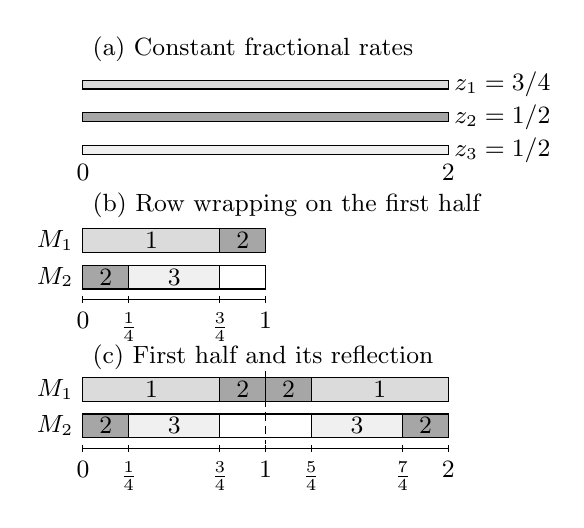
\begin{tikzpicture}[x=2.32cm,y=0.63cm,font=\small]
 \node[anchor=west] at (0,9.05) {(a) Constant fractional rates};
 
 \foreach \y/\rate/\job/\shade in {8.25/{3/4}/1/14,7.59/{1/2}/2/35,6.93/{1/2}/3/6}{
   \draw[fill=black!\shade] (0,\y) rectangle (2,{\y+.18});
   \node[anchor=west,inner sep=2pt] at (2,{\y+.09}) {$z_\job=\rate$};
 }
 \node[below,inner sep=1pt] at (0,6.79) {$0$};
 \node[below,inner sep=1pt] at (2,6.79) {$2$};
 \node[anchor=west] at (0,5.9) {(b) Row wrapping on the first half};
 \foreach \y/\mach in {4.95/1,4.22/2}{
   \draw (0,\y) rectangle (1,{\y+.48});
   \node[anchor=east] at (0,{\y+.24}) {$M_{\mach}$};
 }
 \draw[fill=black!14] (0,4.95) rectangle node {$1$} (.75,5.43);
 \draw[fill=black!35] (.75,4.95) rectangle node {$2$} (1,5.43);
 \draw[fill=black!35] (0,4.22) rectangle node {$2$} (.25,4.70);
 \draw[fill=black!6] (.25,4.22) rectangle node {$3$} (.75,4.70);
 \foreach \x/\labeltext in {0/0,.25/{\tfrac14},.75/{\tfrac34},1/1}{
   \draw (\x,4.08) -- (\x,3.94);
   \node[below] at (\x,3.94) {$\labeltext$};
 }
 \draw (0,4.01) -- (1,4.01);
 \node[anchor=west] at (0,2.84) {(c) First half and its reflection};
 \foreach \y/\mach in {1.95/1,1.22/2}{
  \draw (0,\y) rectangle (2,{\y+.48});
  \node[anchor=east] at (0,{\y+.24}) {$M_{\mach}$};
 }
 \draw[fill=black!14] (0,1.95) rectangle node {$1$} (.75,2.43);
 \draw[fill=black!35] (.75,1.95) rectangle node {$2$} (1,2.43);
 \draw[fill=black!35] (1,1.95) rectangle node {$2$} (1.25,2.43);
 \draw[fill=black!14] (1.25,1.95) rectangle node {$1$} (2,2.43);
 \draw[fill=black!35] (0,1.22) rectangle node {$2$} (.25,1.70);
 \draw[fill=black!6] (.25,1.22) rectangle node {$3$} (.75,1.70);
 \draw[fill=black!6] (1.25,1.22) rectangle node {$3$} (1.75,1.70);
 \draw[fill=black!35] (1.75,1.22) rectangle node {$2$} (2,1.70);
 \draw[densely dashed] (1,2.57) -- (1,1.10);
 \draw (0,1.01) -- (2,1.01);
 \foreach \x/\labeltext in {0/0,.25/{\tfrac14},.75/{\tfrac34},1/1,1.25/{\tfrac54},1.75/{\tfrac74},2/2}{
   \draw (\x,1.08) -- (\x,.94);
   \node[below] at (\x,.94) {$\labeltext$};
 }
\end{tikzpicture}
\caption{Reflected realization on two machines. The cells are labeled by job and blank cells are idle. Job~2 wraps between the two rows in the first half. Reflection about time~1 keeps each operation on its assigned machine.}\label[figure]{fig:reflection}
\end{figure}


Ordinary wrapping over the full interval can change individual moments. For $[0,1]$, one machine and rates $(1/2,1/2)$, both fractional first moments are $1/4$. Serving job 1 on $[0,1/2)$ followed by job 2 on $[1/2,1)$ gives first moments $(1/8,3/8)$. With coefficients $(1,2)$ the fractional cost is $3/4$, compared with $7/8$ for that order and $5/8$ for its reverse. Reflection makes each job's first moment equal to its workload times the phase midpoint.

\section{An exact certificate for Queyranne's example}\label[section]{sec:example}

Queyranne gives three unit-work jobs on two machines with raw coefficients $(11,10,9)$ \cite[p.~16]{queyranne2010}. Use the following half-open operations, with no other activity. The schedule in \Cref{fig:benchmark} uses the same assignments.
\begin{center}
\begin{tabular}{@{}ccc@{}}
\toprule
Machine & Job & Interval \\
\midrule
$1$ & $1$ & $[0,1)$\\
$1$ & $2$ & $[1,29/20)$\\
$2$ & $2$ & $[0,11/20)$\\
$2$ & $3$ & $[11/20,31/20)$\\
\bottomrule
\end{tabular}
\end{center}
Job 1 receives unit work. Job 2 receives $11/20+9/20=1$ on disjoint intervals, and job 3 receives $(31-11)/20=1$. Using one half of the difference of squares on each operation gives the moment vector
\[
 \left(\tfrac12,\ \tfrac12\bigl((11/20)^2+(29/20)^2-1\bigr),\
                   \tfrac12\bigl((31/20)^2-(11/20)^2\bigr)\right)
       =\left(\tfrac12,\tfrac{281}{400},\tfrac{21}{20}\right).
\]
Thus the objective is $11/2+10(281/400)+9(21/20)=879/40=21.975$.

\begin{figure}[tbp]
\centering
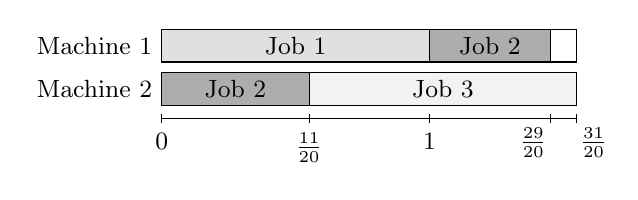
\begin{tikzpicture}[x=3.4cm,y=.72cm,font=\small]
 \draw (0,1.3) rectangle (1.55,1.88);
 \draw (0,.54) rectangle (1.55,1.12);
 \node[anchor=east] at (0,1.59) {Machine 1};
 \node[anchor=east] at (0,.83) {Machine 2};
 \draw[fill=black!12] (0,1.30) rectangle node {Job 1} (1,1.88);
 \draw[fill=black!32] (1,1.30) rectangle node {Job 2} (1.45,1.88);
 \draw[fill=black!32] (0,.54) rectangle node {Job 2} (.55,1.12);
 \draw[fill=black!5] (.55,.54) rectangle node {Job 3} (1.55,1.12);
 \draw (0,.30) -- (1.55,.30);
 \foreach \x in {0,.55,1,1.45,1.55}{
   \draw (\x,.38) -- (\x,.22);
 }
 \node[below] at (0,.22) {$0$};
 \node[below] at (.55,.22) {$\tfrac{11}{20}$};
 \node[below] at (1,.22) {$1$};
 \node[below left,inner sep=1pt] at (1.45,.20) {$\tfrac{29}{20}$};
 \node[below right,inner sep=1pt] at (1.55,.20) {$\tfrac{31}{20}$};
\end{tikzpicture}
\caption{Optimal operations for the three-job, two-machine example. Job~2 migrates between machines after an interruption. Both machines are idle from $31/20$ onward.}\label[figure]{fig:benchmark}
\end{figure}


For a dual certificate take $\lambda=(31/2,29/2,279/20)$ and $H=6$. With $c_j(t)=\lambda_j-t\alpha_j$, the following sets maximize the support at \emph{both} endpoints of each indicated interval. The table is obtained by evaluating all three rational scores and choosing up to two positive values, allowing zero-score jobs and ties.
\begin{center}
\begin{tabular}{@{}ccc c@{}}
\toprule
Interval & Maximizing jobs & Left support & Right support\\
\midrule
$[0,11/20]$      & $\{1,2\}$ & $30$      & $369/20$\\
$[11/20,1]$      & $\{1,3\}$ & $369/20$ & $189/20$\\
$[1,29/20]$      & $\{2,3\}$ & $189/20$ & $9/10$\\
$[29/20,31/20]$  & $\{3\}$   & $9/10$   & $0$\\
$[31/20,6]$      & $\varnothing$ & $0$  & $0$\\
\bottomrule
\end{tabular}
\end{center}
For example, at $11/20$ jobs 2 and 3 tie at $9$ while job 1 scores $189/20$. At $1$, jobs 1 and 2 tie at $9/2$ and job 3 scores $99/20$. The endpoint-maximization argument of \Cref{sec:recovery} permits exact trapezoid integration on each interval. It gives
\[
 J(\lambda)=\tfrac{10659+5022+1863+36}{800}
            =\tfrac{879}{40}.
\]
The scores at $H$ are nonpositive and remain so thereafter. Since $\lambda\cdot p=879/20$, the bound \eqref{eq:bound} is $879/40$. The displayed schedule attains it among all feasible measurable schedules. The exact Lean benchmark uses the same instance and endpoint support assignments, with scalar thresholds witnessing their maximization.
 In the order of the table, valid endpoint-threshold pairs are
\[
 (29/2,9),\quad (9,9/2),\quad (9/2,0),\quad (0,0),\quad (0,0).
\]

\section{Formal verification and reproducibility}\label[section]{sec:formal}

\paragraph{Scheduling and realization.}
The Lean model uses extended nonnegative costs on the real half-line and binary activity almost everywhere. In the namespace \leanid{TBB.MeasurableSchedule}, the predicate \leanid{Feasible} specifies workload and capacity, and \leanid{normalizedCost_eq_cost} and its converse give the coefficient conversion in \Cref{sec:model}. Theorems \leanid{labeled_feasible} and \leanid{labeled_same_cost} connect measurable activities with labeled machine assignments and their costs.

In the namespace \leanid{TBB}, \leanid{reflected_realization} verifies the construction for nonnegative times, and \leanid{reflected_realization_on_line} covers intervals on the full real line. The guarantees include machine and job nonoverlap, per-job rational workload and moment identities, and the $4nq$ record bound. The machine bound follows from \leanid{TBB.realizePhase_machine_min}. The bridge lemma \leanid{realize_phase_measurable} gives the Lebesgue integral identities for a phase at nonnegative times, and \leanid{realize_measurable_totals} sums them.

\paragraph{Certificate checker.}
The input is a typed rational record with instance data, a finite schedule partition (including idle pieces), a candidate multiplier, and the claimed moments and objective. At each phase endpoint the implementation checks a rational scalar threshold. For scores $c$ and $\theta\geq0$, any $u\in P$ satisfies
\[
 c\cdot u \leq m\theta+\sum_{j=1}^n\max(c_j-\theta,0).
\]
Indeed subtract $\theta$ from each score, bound the positive terms by the unit rate caps and use the capacity bound for the $\theta$ term. Equality for the phase assignment certifies that it is a maximizer. The checker combines endpoint inequalities by affine interpolation and checks the tail sign condition. It also verifies dimensions and index ranges, positive data, the phase partition, assignment compatibility, exact work, moments, and primal--dual equality.

The theorem \leanid{TBB.check_sound} turns acceptance of a raw rational certificate into a decoded certificate and its soundness proof. The predicate \leanid{TBB.Certificate.Sound} includes feasibility, exact moments and cost, and optimality over arbitrary feasible measurable competitors. Its theorem \leanid{optimal_aeActivity} covers activities measurable for the completed measure. The proof compares against competitors running past the certificate horizon, and extended nonnegative costs accommodate infinite-cost competitors. The guarantee is for the instance actually encoded by the certificate. Matching those fields to an intended instance is the user's responsibility. The JSON adapter used in bulk experiments is outside the trusted mathematical proof path.

\paragraph{Benchmark and private verification.}
\leanid{TBB.benchmark_accepts} proves acceptance through Lean kernel reduction. \leanid{TBB.benchmark_optimal} derives the global optimality statement for the value $879/40$. The supplement includes the typed benchmark and audit instructions. The current verification uses Lean 4.36.0 and Mathlib revision
\begin{center}
 \texttt{\small fc4f59e577feb1a4956671bc04ac18aaaf8cd842}.
\end{center}
The manifest pins the transitive dependencies. We rebuilt the project modules and validated the 52 audit declarations and their exported proof dependencies with the patched Lean kernel and independent kernels including nanoda.

An independent AI review of the historical Lean 4.19.0 build reproduced a clean source build of 2{,}274 modules with zero errors. The audit of 52 declarations reported only \texttt{propext}, \texttt{Classical.choice}, and \texttt{Quot.sound}. The audited project source contains no proof placeholders, project-defined axioms, or uses of \leanid{native_decide} or unsafe code. During private verification the review reproduced 79 archived optimality-certificate checks, 1{,}553 archived realization checks and 23 archived negative controls. Additional private checks covered constructor replay on the 1{,}553 realization inputs and two further cases, and 329{,}890 Node verifier assertions. The AI referee independently generated 123 certificates that the checker accepted and 62 adversarial corruptions that it rejected. These bulk results are executable evaluations. The benchmark acceptance and optimality statements are kernel-verified. The extended inputs and replay tools are retained privately.

\paragraph{Scope.}
Theorem~Q, the GLS-based optimization procedure, its bit-complexity proof, and the full optimizer-to-certificate chain are conventional mathematics. The full theoretical GLS optimizer has not been implemented. The executable checker certifies a supplied witness independently of the method used to obtain it.

\section{Limitations and conclusion}\label[section]{sec:conclusion}

The running-time guarantee is weakly polynomial. It uses general exact polyhedral optimization, and the explicit description bound is intended for a worst-case proof. The model assumes identical unit-speed machines, common release at zero, positive rational coefficients and free preemption and migration. It makes no allowance for setup, migration costs, job-specific release dates, or machine eligibility. Simpler exact algorithms and sharper complexity guarantees remain natural questions.

For a variable number of machines, exact dual recovery followed by reflected realization yields a rational optimal schedule and certificate in polynomial bit time. The realization and certificate soundness are machine-checked independently of the optimizer. The latter permits exact certification even when the schedule is obtained by another method. The comparisons in \Cref{sec:related} delimit the evidence on priority.

\section*{Research transparency and availability}

\paragraph{AI-assisted research.}
This work was developed under The Blank Beyond through an AI-assisted research process. AI systems contributed substantially to mathematical investigation, proof development, computational verification, Lean formalization, adversarial review, and manuscript preparation. A separate AI system, Claude, reviewed the conventional arguments and revisions, rebuilt the formalization, and reproduced the scoped Lean verification. The Blank Beyond directed the work and prepared it for private review. That editorial role, independent AI review, and machine-checked proofs are distinct from independent human academic peer review, which has not occurred.

\paragraph{Software and evidence availability.}
The supplement designated for public release contains the scoped Lean proofs, exact rational checker, typed three-job benchmark, pinned dependencies, and build and audit instructions. With these files readers can rebuild the formalization, reproduce the axiom audit, and verify the kernel proofs of benchmark acceptance and optimality at $879/40$. The manuscript contains the complete conventional proof, including the mathematical optimizer specification and encoding analysis. The extended corpora, bulk replay tools and practical producer are retained privately. The private verification results reported in \Cref{sec:formal} are supplementary evidence.

\appendix
\section{Explicit rational encoding bounds}\label[appendix]{app:encoding}

We give a computable GLS row-length promise and bound the time and size of the operations that use it. Throughout, $n\leq L$. For a reduced rational $a/b$ with $b>0$, a component bound $B\geq1$ means $|a|,b<2^B$. Product bounds add, and reciprocation of a nonzero rational and negation preserve the bound. For a sum of at most $k$ signed rationals of component bound $B$ use
\[
 S(k,B)=kB+\lceil\log_2(k+1)\rceil+2 .
\]
The product of the $k$ denominators bounds the denominator, and each term after clearing it has magnitude less than $2^{kB}$. The estimate holds also for partial sums, with reduction at each operation. Integer arithmetic, exact comparison and reduction by gcd take polynomial bit time on the indicated lengths.

GLS charges $1+\lceil\log_2(|a|+1)\rceil$ bits for a signed integer $a$ \cite[\S1.3, pp.~29--30]{gls1988}. A reduced rational costs the sum for its numerator and denominator. A scalar with bound $B$ costs at most $2B+2$ bits, a $d$-vector at most $d(2B+2)$, and a row with right-hand side at most $(d+1)(2B+2)$. Matrices and explicit systems sum these lengths. An equation can be given by two opposing rows.

\subsection{Vertices of rational systems}
For $d\geq1$ define
\[
 D(d,B)=d(d+1)B+d\lceil\log_2(d+1)\rceil+2.
\]
At a vertex of a finite rational system, $d$ independent tight rows exist, since a smaller active rank would permit a feasible displacement in both signs. If each entry, including the right side, has component bound $B$, clearing denominators separately in these $d$ rows bounds the integer entries by $2^{(d+1)B}$ in magnitude. Each determinant in Cramer's rule is bounded by $d!2^{d(d+1)B}$. Hence each vertex coordinate has bound $D(d,B)$. A nonempty pointed polyhedron has a vertex. Start at any point of rank less than $d$ and take a nonzero direction in the active nullspace. Pointedness implies that some row does not annihilate it. Choose its sign to meet a new constraint by following it until the first such constraint becomes tight. The active rank strictly increases, because the new row does not annihilate the direction. This proves existence up to rank $d$, also for lower-dimensional or unbounded systems, with no need for an active-set enumeration.

\subsection{Description of the minimizer polytope}
Put $b=L+4$. The input workloads, input weights, $n$ and $m_\star$ have component bound $b$, and $\alpha$ has bound $2b$, allowing the division for normalized weights. Computing $m_\star$ uses the binary $m$ directly. Bounds for $V$, $H$, and each $\alpha_jV$ are $S(n,b)$, $S(n,b)+1$, and $2b+S(n,b)$. Set
\[
 E=S(n,b)+4b+8,\qquad B_A=S(2,E).
\]
Since $\alpha_i-\alpha_j$ has bound $S(2,2b)\leq4b+4$, the affine events in \Cref{lem:envelope} have every coefficient, including the constant, bounded by $E$. The arrangement walls and box rows in \Cref{lem:polytope} are oriented comparisons with component bound $B_A$ and row length at most $(n+1)(2B_A+2)$.

For the rational quadratic on each cell, set
\begin{align*}
 T_0 &= q_0\bigl(2n(n+1)+2(n+1)^2\bigr)+n,\\
 B_Q &= S\bigl(T_0,\,2E+S(n,2b)+3\bigr)+4 .
\end{align*}
In \eqref{eq:integral-piece}, the linear score times the endpoint difference contributes at most $2n(n+1)$ terms to the monomial expansion on each interval. The endpoint squares contribute at most $2(n+1)^2$ terms with factors from $\alpha\cdot v_\ell$, and subtracting $\lambda\cdot p$ adds $n$. The component bound inside $S$ follows from the product rule. The spare four bits cover conversion to the entries of $Q_C,d_C$, including the diagonal factor of two. The same coefficients represent the function on the closure.

The system \eqref{eq:kkt} has at most $2n$ variables and rows with coefficients from $A,b,Q_C,d_C,0,\pm1$. Its nonempty pointed form gives a rational $x_C$ with coordinate bound
\[
 B_0=D(2n,\max\{B_A,B_Q\}).
\]
The minimizer equations \eqref{eq:cell-min} then have rows bounded by using
\begin{align*}
 B_g &= S(n+1,B_Q+B_0),\\
 B_C &= \max\{B_A,B_Q,S(n,B_Q+B_0),B_g,S(n,B_g+B_0)\},\\
 B_* &= D(n,B_C).
\end{align*}
Here $B_g$ bounds $Q_Cx_C+d_C$. The dot-product right sides in \eqref{eq:cell-min} are covered by $S(n,B_Q+B_0)$ and $S(n,B_g+B_0)$. Thus $B_*$ bounds every vertex coordinate of every cell minimizer polytope. By \Cref{lem:polytope} it also bounds every vertex coordinate of $K^*$. The total length of each vertex vector is at most $\nu=n(2B_*+2)$. GLS Lemma~(6.2.4)(b) \cite[pp.~164--165]{gls1988} gives the computable whole-row bound
\begin{equation}\label{eq:F}
 F=3n^2\nu .
\end{equation}

For a direct affine-hull bound, let $k$ be its dimension and choose $k+1$ affinely independent vertices spanning it. The $k$ difference vectors against a base vertex have coordinate bound $S(2,B_*)$. Select $k$ pivot columns. To construct a basis of normals, set one free coordinate to one, the other free coordinates to zero, and solve the pivot system for each choice. Cramer's rule gives the bound $B_\perp=D(n,S(2,B_*))$, with unit normals when $k=0$ and no normals when $k=n$. The affine-hull equations have right sides given by dot products with the base vertex, so each whole row in either sign has length at most
\[
 (n+1)\bigl(2\max\{B_\perp,S(n,B_\perp+B_*)\}+2\bigr).
\]
Independently GLS (6.2.3) gives a standard-form bound $35n^2F$ for affine-hull equations and relative-facet rows. These are existence estimates. Denominators are cleared within sums or individual systems and can differ across cells. The algorithm does not generate the global row or vertex lists.

\subsection{Oracle computations and exact LP}
Let $T$ be the length of a rational query in the original $n$ coordinates. The exact rational evaluation, sorting, and midpoint construction of the time events have bounds
\begin{align*}
 B_t(T)&=S(n+1,E+T+2),&
 B_\Delta&=S(2,B_t(T)),&
 B_{\mathrm{mid}}&=B_\Delta+1 .
\end{align*}
For midpoint score components use $B_s=S(2,\max\{T,B_{\mathrm{mid}}+2b\})$. The support value there costs a sum of at most $n$ such components. Thus every \FaceLP{} coefficient and right side has component bound
\[
 B_{\mathrm{LP}}(T)=\max\{B_\Delta,B_s,S(n,B_s),b\}.
\]
With $N_r=nr$ variables, there are $2nr$ box rows, $r$ capacity rows, $2r$ support-face rows, and $2n$ workload rows when expressing equations in both signs. Each variable is bounded by its box. The dense rational LP including a zero objective has length at most
\[
 (2nr+3r+2n)(N_r+1)(2B_{\mathrm{LP}}(T)+2)+2N_r
\]
plus polynomial dimensional framing. GLS Theorem~(6.4.12) gives exact feasibility and a point if feasible, including for lower-dimensional feasible sets.

Outside the box the query is separated by a signed coordinate normal. When \FaceLP{} is infeasible at a query in the box, the mismatch $g$ has coordinate bound $B_{\mathrm{cut}}=S(q_0+1,\max\{B_\Delta,b\})$. Its positive max norm is a rational magnitude of one coordinate. The normalized separator has total size at most $n(4B_{\mathrm{cut}}+2)$. Construction of the envelope uses $O(n^2\log(n+1)+nq_0\log(n+1))$ rational comparisons. Formation of the LP, its exact solution, and all remaining arithmetic and comparisons take bit time polynomial in $L+T$. The oracle uses no approximation of the unknown minimum value.

\subsection{Implicit and explicit recovery}
For the question-length convention of GLS \cite[(1.2.1), pp.~26--27]{gls1988}, provide the implicit optimizer with $K^*\times\{0\}^L$ in dimension $n+L$ with bound $F+4L$. Zero coefficients add at most $4L$ bits per row and the added zero equations fit the same bound. At a rational query, check the added coordinates and either separate by a signed coordinate vector or extend the original separator by zeros. A padded query has length at least $L$ so the original runtime and reply bound, polynomial in $L+T$, are bounded by a fixed polynomial in the question length alone. Padded optimization objectives also have zero new coordinates.

For successive multiplier minima the sets are exposed faces, hence the fixed values have bound $B_*$. Their prefix equations can be added with the uniform bound
\[
 F'=\max\{F,(n+1)(2B_*+2)\}
\]
before padding. Strong optimization queries the augmented oracle with input length bounded by $n+L+F'+4L$ plus the length of a coordinate objective. The number of oracle calls and lengths of written queries are polynomial in that input length. Implementing the oracle as above therefore gives ordinary deterministic polynomial Turing bit time. The final multiplier has length at most $T_*=n(2B_*+2)$. No approximate minimizer is rounded to obtain it.

Apply the same successive-coordinate method to \FaceLP{} at $\lambda^*$. Each new constraint fixes the coordinate of an original LP vertex, so the right sides and newly formed explicit LPs have polynomial encoding throughout. After at most $nr$ exact LP calls, each coordinate of the returned vertex satisfies
\[
 B_z=D(nq_0,B_{\mathrm{LP}}(T_*)).
\]
These rate-recovery calls are used only at $\lambda^*$ and are separate from the feasibility calls in the oracle.

\subsection{Schedule and certificate}
Put $N=nq_0$, $B_t=B_t(T_*)$, $B_h=S(2,B_t)+1$ and $B_\Sigma=S(n,B_h+B_z)$. These bound the event endpoints, half-lengths and cumulative half-work lengths, respectively. In \Cref{thm:r}, a local row endpoint is obtained from a cumulative work boundary and a row boundary $kh$, with $k\leq n$, or is $0$ or $h$. Translation by $a_\ell$ therefore gives a first-half endpoint bound $B_e'=S(3,\max\{B_t,B_\Sigma,B_h+b\})$. A reflected endpoint is $a_\ell+b_\ell-e$, so a bound for all endpoints is $B_e=S(3,\max\{B_t,B_e'\})$. There are at most $4N$ nonempty operations, and at most $8N+2$ global event intervals including idle pieces up to $H$. Every preemption occurs at an operation boundary. The construction, sorting and sweep use polynomially many exact operations and work only with occupied rows. A machine-operation record costs at most $2(2B_e+2)+2(b+1)$ bits before framing. Listing all active assignments multiplies the event count by at most $n$.

An operation moment has bound $B_{\mathrm{mom}}=S(2,2B_e)+1$. The objective has bound $S(4N,B_{\mathrm{mom}}+2b)$ and the multiplier has length at most $T_*$. For verification, \eqref{eq:integral-piece} uses dot products with at most $n$ entries, interval lengths and endpoint squares. The polynomial bound on these operands, the at most $q_0$ terms, and the exact rational checks of nonoverlap, workloads, moments, and equality prove the certificate bound. The same operations are polynomial in the actual encoded length of a supplied certificate.

Each bound is polynomial in $L$, including the dimension and time-event counts. The dependence on binary input length gives weakly polynomial bit complexity. The operation counts alone would not establish this result. Neither discretization in time nor the generation of all subsets, chambers or active sets is used.

\section{Exact polyhedral optimization contracts}\label[appendix]{app:gls}

We use the following results of the 1988 first edition of Gr\"otschel, Lov\'asz and Schrijver \cite{gls1988}. Page numbers refer to its printed pagination.

\begin{itemize}
 \item Definition (6.2.2), p.~163. A rational polyhedron with facet complexity at most $F$ admits a system of rational inequalities with full row lengths at most $F$. A \emph{well-described polyhedron} is a triple $(P;d,F)$ of encoding length $d+F$. The promised description need not be supplied. A vertex complexity bound controls the length of each vector in finite vertex and ray generating lists. For a compact polytope the ray list is empty.
 \item Strong separation, (2.1.4), p.~48 and \S6.2, p.~163. On rational $y$ the oracle affirms membership or returns a rational $c$ with $c^Ty>c^Tx$ for all $x$ in the set. A unit norm is not required by (2.1.4). Our oracle supplies $\|c\|_\infty=1$ also, as obtained by positive rational scaling in the non-coordinate case. Compare the weak separation normalization in (2.1.13), p.~51.
 \item Lemma (6.2.4), pp.~164--165. Facet complexity at most $F$ implies vertex complexity at most $4d^2F$. Vertex complexity at most $\nu$ implies facet complexity at most $3d^2\nu$, including for lower-dimensional polyhedra.
 \item Theorem (6.4.1), pp.~174--178. Given a well-described polyhedron by strong separation, one can decide emptiness and return an exact rational feasible point in oracle-polynomial time. No ambient interior is required.
 \item Theorem (6.4.9), pp.~179--180. Strong separation, strong violation, and strong linear optimization for a well-described polyhedron are mutually oracle-polynomially reducible. Strong linear optimization has a rational linear objective and returns an exact optimizer, emptiness, or a direction of unbounded increase as appropriate.
 \item Theorem (6.4.12), pp.~180--181. A linear program given by explicit rational matrix, right side and objective can be solved in time polynomial in their encoding, with exact rational recovery in the feasible bounded case.
\end{itemize}

Here nonemptiness of the implicit set follows from attained duality in \Cref{lem:compression}. \Cref{lem:polytope} proves rationality in the ambient space and \eqref{eq:F} supplies the required promise, including affine-hull constraints. No interior assumption on $K^*$, on its prefix faces, or on \FaceLP{} is used. All of these are bounded. The oracle in \Cref{lem:separate} tests exact membership and satisfies the strict inequality, and the prefix and padding oracles preserve it by the coordinate tests. \Cref{app:encoding} bounds the input, written queries, reply encodings and exact subroutine time in the oracle-Turing model of \cite[\S1.2, pp.~26--27]{gls1988}. The multiplier and rate recovery described there provides finite rational coordinates by exact optimization under these contracts.

\bibliographystyle{amsplain}
\bibliography{references}
\end{document}
